\documentclass{article}
\usepackage{pgfplots}
\pgfrealjobname{echo}
\pgfplotsset{compat=newest}

\begin{document}

\beginpgfgraphicnamed{echo-f0}
% time ./echo_server_client 1000 5000
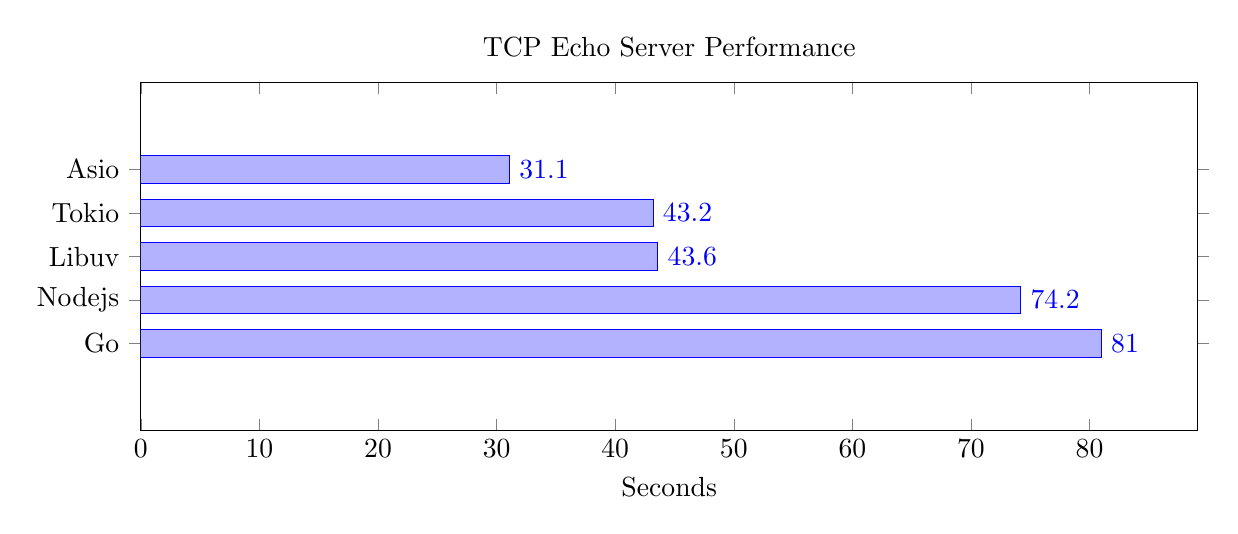
\begin{tikzpicture}[scale=1.0]
  \begin{axis}[
    y dir=reverse,
    %xbar stacked,
    xbar, xmin=0,
    %hide x axis,
    bar shift=0pt,
    width=15cm, height=6cm, enlarge y limits=0.5,
    title={TCP Echo Server Performance},
    xlabel={Seconds},
    symbolic y coords={Asio,Tokio,Libuv,Nodejs,Go},
    ytick=data,
    %bar width=1cm,
    nodes near coords,
    nodes near coords align={horizontal},
    ]
    \addplot coordinates {
       (31.1,Asio)
       (43.2,Tokio)
       (43.6,Libuv)
       (74.2,Nodejs)
       (81.0,Go)
    };
  \end{axis}
\end{tikzpicture}
\endpgfgraphicnamed

\beginpgfgraphicnamed{echo-f1}
%debian2[0]$ time ./echo_server_client 1000 1000
%Go  (1):   1.000s
%C++ (1):   0.07s
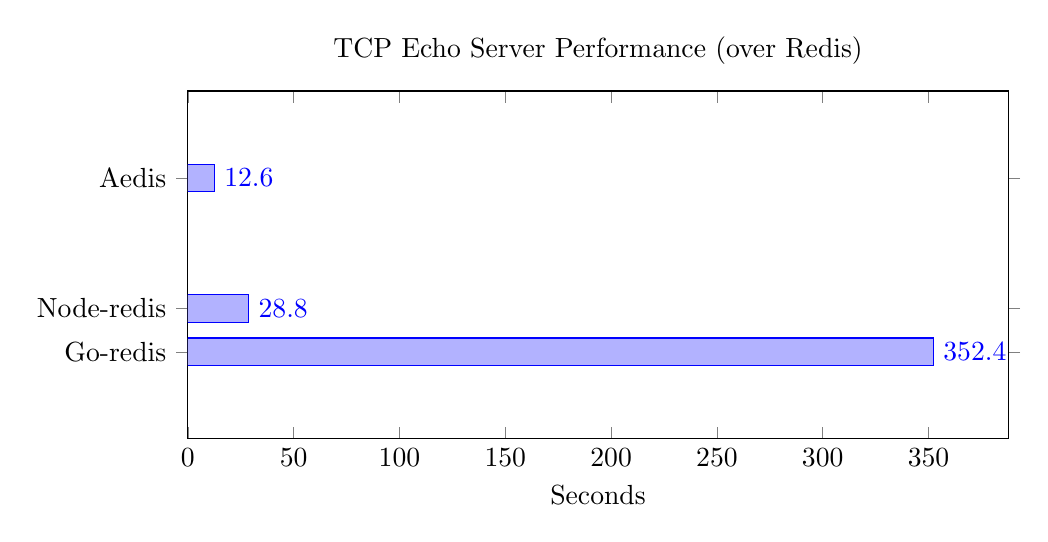
\begin{tikzpicture}[scale=1.0]
  \begin{axis}[
    y dir=reverse,
    %xbar stacked,
    xbar, xmin=0,
    %hide x axis,
    bar shift=0pt,
    width=12cm, height=6cm, enlarge y limits=0.5,
     title={TCP Echo Server Performance (over Redis)},
    xlabel={Seconds},
    symbolic y coords={Aedis,Rust-rs,Libuv,Node-redis,Go-redis},
    ytick=data,
    %bar width=1cm,
    nodes near coords,
    nodes near coords align={horizontal},
    ]
    \addplot coordinates {
       (12.6,Aedis)
       (28.8,Node-redis)
       (352.4,Go-redis)
    };
    %\addplot coordinates {
    %   (30.0,Asio)
    %   (90.6,Rust-rs)
    %   (0.0,Libuv)
    %   (68.9,Nodejs)
    %   (0.0,Go)
    %};
  \end{axis}
\end{tikzpicture}
\endpgfgraphicnamed

\end{document}
